\apendice{Documentación de usuario}
\section{Introducción}
En este apartado se van a detallar cuales son los requisitos de los usuarios que utilizarán la aplicación web, las instalaciones necesarias para la utilización de la misma (que en este caso no hay ninguna) y un manual de usuario en el que se expondrán las funcionalidades que tiene la web en sus respectivas ventanas. De esta manera, el usuario no tendrá ningún inconveniente a la hora del uso de la web del proyecto.
\section{Requisitos de usuarios}
Los requisitos que deben tener los usuarios para poder utilizar la web son los siguientes:

\begin{itemize}
\item Disponer de conexión a internet para poder acceder al dominio de la web.
\item Disponer de un dispositivo de escritorio o móvil.
\item Los dispositivos mencionados anteriormente deberán tener un navegador actualizado para garantizar una buena compatibilidad.
\item Contar con una cuenta de correo electrónico activa para poder recibir los avisos. Este requisito no es imprescindible para el uso de la web pero si necesario si se quiere disponer de la funcionalidad de la aplicación al completo.
\end{itemize}
\section{Instalación}
Dado que el proyecto ha consistido en realizar una aplicación web. Tan solo es necesario tener un navegador web para poder acceder a ella, este navegador web deberá estar actualizado para evitar problemas de compatibilidad. 

Ninguna instalación es necesaria ya que la aplicación se encuentra desplegada en un servidor remoto y por lo tanto cualquier usuario podrá acceder a ella desde su dispositivo. El enlace completo para acceder a la web es el siguiente:

\url{https://deltaoffers.azurewebsites.net/}\label{enlace:web}.

\section{Manual del usuario}
En esta sección, se van a proporcionar instrucciones sobre el uso de la aplicación para que los usuarios puedan explotar sus funcionalidades al máximo.

Este manual de usuario se puede seguir en tiempo real a la vez que se utiliza la web, de esta forma el usuario entenderá el uso de la misma de manera más rápida y eficiente. La dirección de la web es aquella que se mostró en el apartado \ref{enlace:web}.

\subsection{Pantalla de inicio}
En esta ventana inicial, el usuario será informado de cuál es el propósito de la web junto con el nombre de esta. En el momento en el que este desee empezar con la utilización de la misma, hará \textit{click} en el botón 'Empieza ya'.
\begin{figure}[H]
    \centering
    
\includegraphics[width=1\linewidth]{DocumentacionTFG//img/VentanaInicial.PNG}
    \caption{Ventana Inicial}
    \label{fig:ventana-inicial}
\end{figure}

\subsection{Visualización convocatorias}
Una vez pulsado el botón 'Empieza ya' el usuario visualizará un listado competo de las convocatorias. Estas convocatorias estarán ordenadas en orden descendiente por la fecha de fin de plazo. En este listado aparecerán las convocatorias en plazo actualmente y las convocatorias cerradas que se muestran más recientes en las webs de las propias universidades.

\begin{figure}[H]
    \centering
    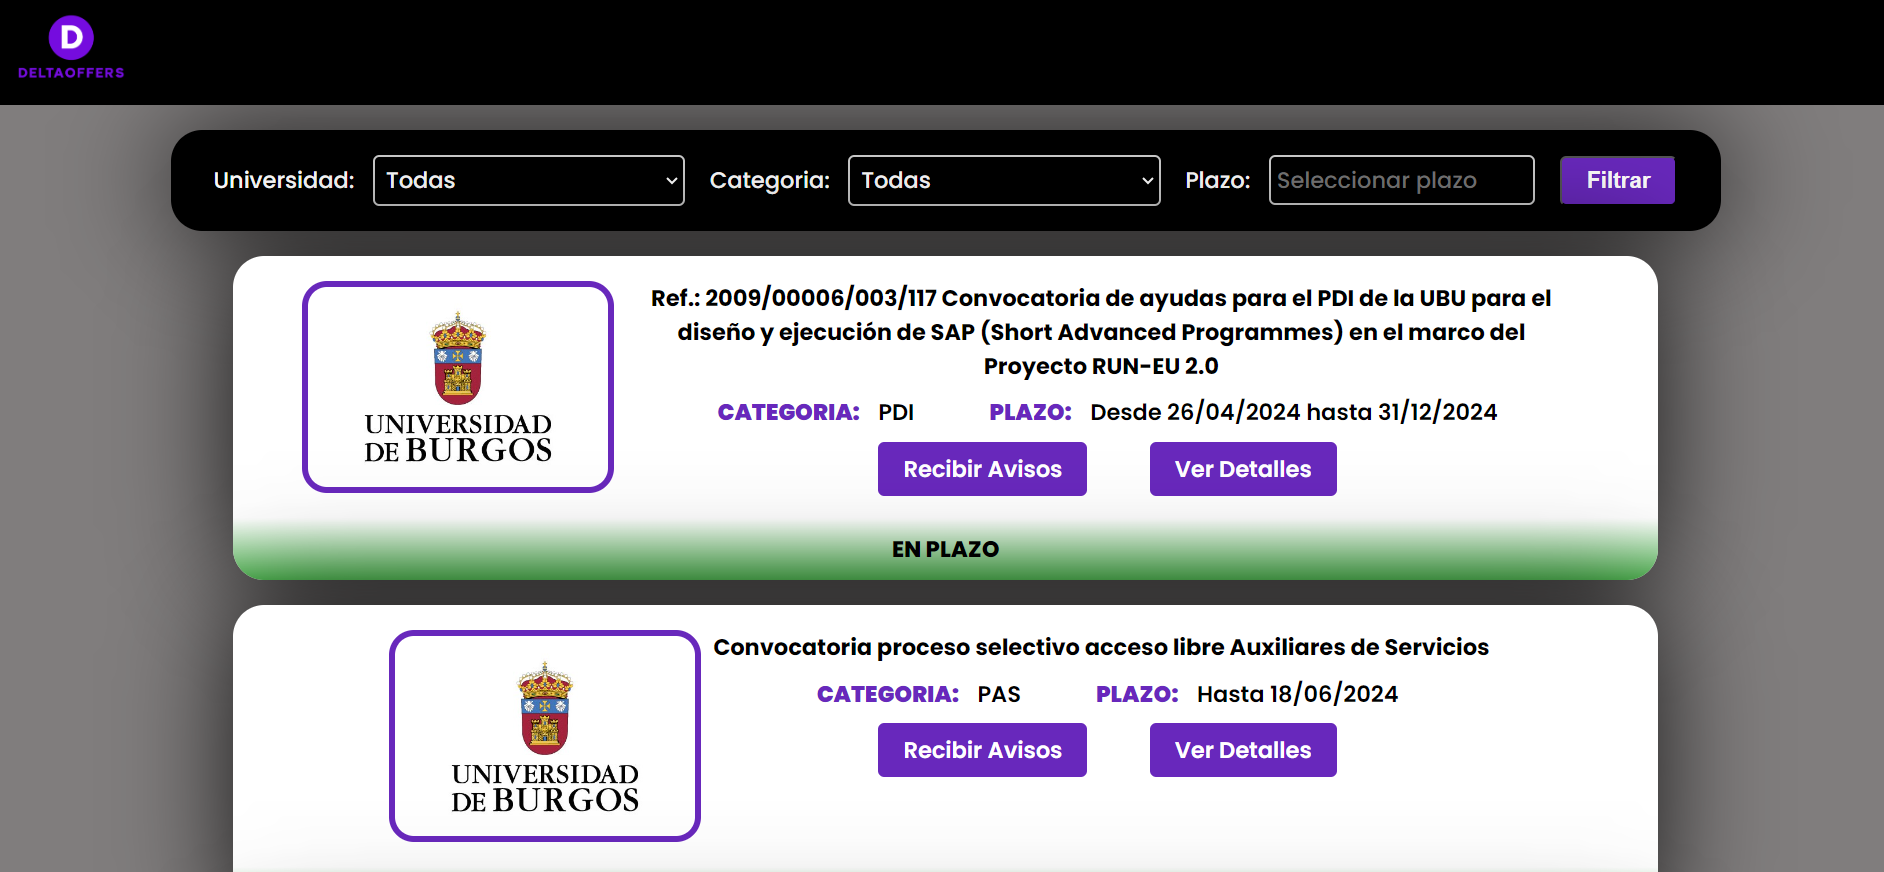
\includegraphics[width=1\linewidth]{DocumentacionTFG//img/VisualizacionConvocatorias.PNG}
    \caption{Visualización convocatorias}
    \label{fig:visualizacion-convocatorias}
\end{figure}

Se podrán visualizar las correspondientes convocatorias haciendo \textit{scroll} en la ventana de visualización y, para facilitar la navegación, se ha implementado que las convocatorias estén paginadas. El paso a la página siguiente se podrá realizar desde el final de la página actual.

\begin{figure}[H]
    \centering
    
\includegraphics[width=1\linewidth]{DocumentacionTFG//img/Paginacion.PNG}
    \caption{Paginación}
    \label{fig:paginacion}
\end{figure}

\subsection{Aplicar filtros}
Cuando comenzamos con el uso de la aplicación, además de visualizarse las convocatorias, es posible aplicar filtros, de esta manera los usuarios podrán encontrar más rápido las convocatorias que sean de su interés. Los filtros aparecerán en un cuadro negro en la parte superior de la ventana.

Para aplicar los filtros se deben de seguir los siguientes pasos:
\begin{enumerate}
   \item Elegimos la universidad por la que queremos filtrar. Si no queremos filtrar por universidad, dejamos la opción 'Todas'. 
   \item Elegimos la categoría deseada. En el caso de que no se quiera aplicar el filtro de categorías, dejamos marcada la opción de todas.
   \item Elegimos la fecha de fin de plazo máxima, al aplicar ese filtro se nos abrirá un calendario para seleccionar la fecha seleccionada. En el caso de que no se quiera aplicar filtro de fecha, lo tenemos que dejar vacío ese \textit{input}. Otra opción sería que hayamos filtrado por fecha y queremos eliminar el filtro, en ese caso, eliminaremos el texto que aparece en el \textit{input} para filtrar por fecha.
   \begin{figure}[H]
    \centering
    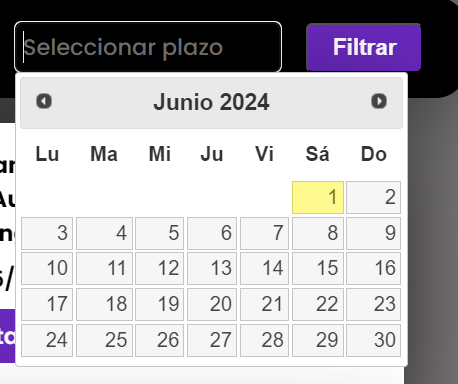
\includegraphics[width=0.5\linewidth]{DocumentacionTFG//img/FiltroCalendario.PNG}
    \caption{Filtro Fecha Fin de Plazo}
    \label{fig:filtro-calendario}
\end{figure}
   \item Finalmente, debemos pulsar el botón 'Filtrar', por el contrario, si este botón no se pulsa, no se aplicarán los filtros y como consecuencia, no nos aparecerán las convocatorias que son de nuestro interés.
\end{enumerate}

\begin{figure}[H]
    \centering
    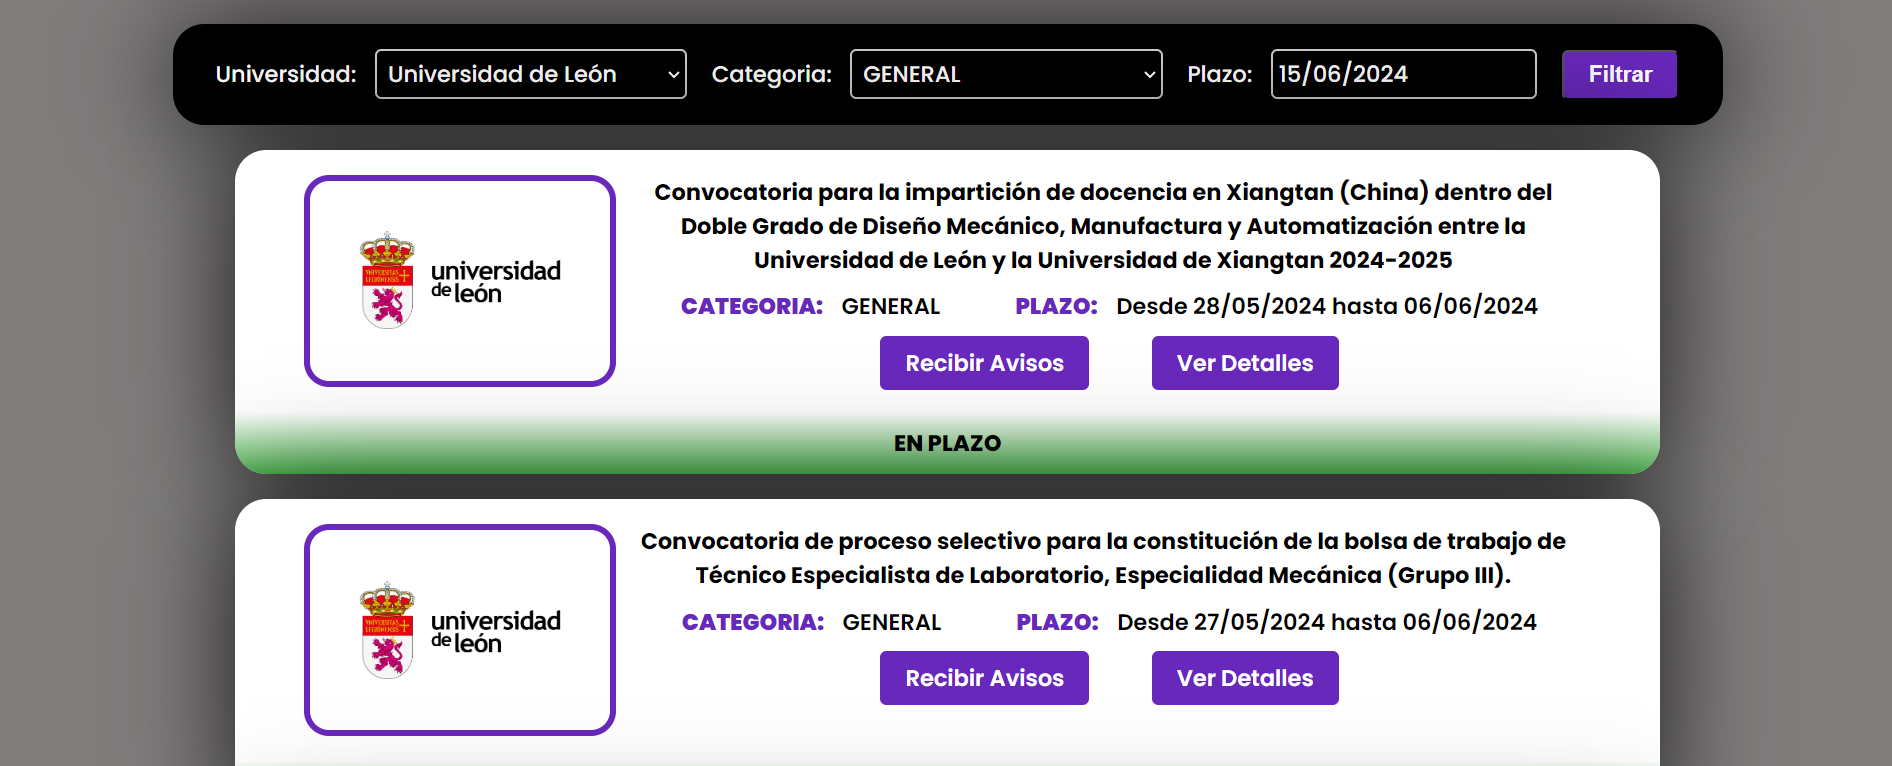
\includegraphics[width=1\linewidth]{DocumentacionTFG//img/AplicarFiltros.PNG}
    \caption{Aplicar filtros}
    \label{fig:aplicar-filtros}
\end{figure}

\subsection{Convocatoria específica}\label{convocatoria-especifica}
En cada convocatoria del listado, aparecerá la siguiente información:
\begin{itemize}
    \item Título de la convocatoria.
    \item Universidad que oferta esa convocatoria.
    \item Categoría de la convocatoria.
    \item Plazo de la convocatoria.
\end{itemize}

Además, aparecerán dos botones los cuales nos permitirán realizar dos labores diferentes:

\begin{itemize}
    \item Suscripción para recibir avisos de las correspondientes convocatorias.
    \item Ver más detalles de esa convocatoria en específico.
\end{itemize}

\begin{figure}[H]
    \centering
    
\includegraphics[width=1\linewidth]{DocumentacionTFG//img/AvisosDetalles.PNG}
    \caption{Convocatoria especifica, avisos y detalles}
    \label{fig:avisos-detalles}
\end{figure}

\subsection{Recibir Avisos}
Una vez que se ha accedido a la sección de recibir avisos para poder recibir los mismos de una convocatoria específica, en primer lugar, nos aparecerá un formulario flotante en el que los usuarios deberán suscribirse con su correo electrónico.

Una vez se introduzca el correo de manera correcta, se pulsa el botón 'Recibir email' para recibir el aviso específico.

En el caso en el que nos aparezca el formulario flotante y queramos salir de él, tan solo tendremos que hacer \textit{click} fuera del formulario y volveremos a la ventana de visualización de convocatorias.

\begin{figure}[H]
    \centering
    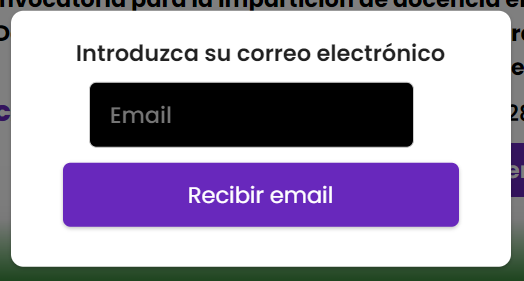
\includegraphics[width=0.5\linewidth]{DocumentacionTFG//img/SuscripcionCorreo.PNG}
    \caption{Suscripción correo}
    \label{fig:suscripcion-correo}
\end{figure}

En el caso de que la suscripción se haya realizado correctamente, el aviso se enviará al correo indicado en el formulario y aparecerá el siguiente mensaje de confirmación en la aplicación:

\begin{figure}[H]
    \centering
    
\includegraphics[width=0.5\linewidth]{DocumentacionTFG//img/CorreoValido.PNG}
    \caption{Correo enviado correctamente}
    \label{fig:correo-enviado}
\end{figure}

Por el contrario, en el caso de que no se haya enviado el correo debido a un error en la suscripción, aparecerá el siguiente error: 

\begin{figure}[H]
    \centering
    
\includegraphics[width=0.5\linewidth]{DocumentacionTFG//img/CorreoNoValido.PNG}
    \caption{Correo no válido}
    \label{fig:correo-no-valido}
\end{figure}

Al aparecer este error, se continuará solicitando rellenar el formulario hasta que la suscripción sea válida y el correo se envíe correctamente o el usuario haga \textit{click} fuera de la ventana flotante en la que está el formulario.

El número de suscripciones mensuales que se pueden realizar tiene un máximo de 5. Puede darse la situación en el que un usuario quiera exceder ese límite, en este caso se mostrará el siguiente error:

\begin{figure}[H]
    \centering
    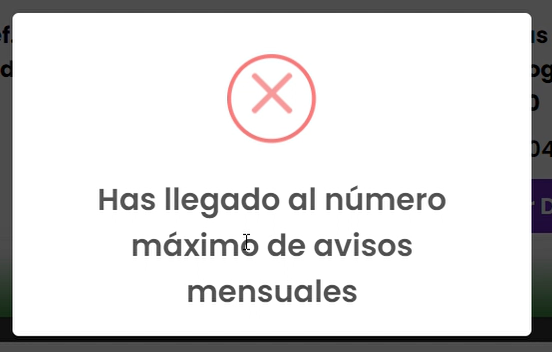
\includegraphics[width=0.5\linewidth]{DocumentacionTFG//img/LimiteSuscripciones.PNG}
    \caption{Limite Avisos Mensuales}
    \label{fig:limite-avisos}
\end{figure}

Al igual que en el caso anterior en el que nos aparecía el error de suscripción no válida, continuará apareciendo el formulario para introducir un correo hasta que se introduzca un correo válido. En el caso de que se quiera salir del envío de formulario, bastará con hacer \textit{click} fuera de la ventana flotante.

\subsection{Añadir al calendario personal}
Una vez aparece en la web la ventana en la que se indica que el correo se ha enviado \ref{fig:correo-enviado}, el usuario deberá iniciar sesión en su correo electrónico personal y verá en la bandeja de entrada un correo cuyo remitente es Delta Offers.

En ese correo, se le notificará al usuario cual es la correspondiente convocatoria de la que ha deseado recibir el aviso y se le adjuntará un archivo ICalendar para añadir un evento a su calendario personal con el fin de plazo de la convocatoria correspondiente.

\begin{figure}[H]
    \centering
    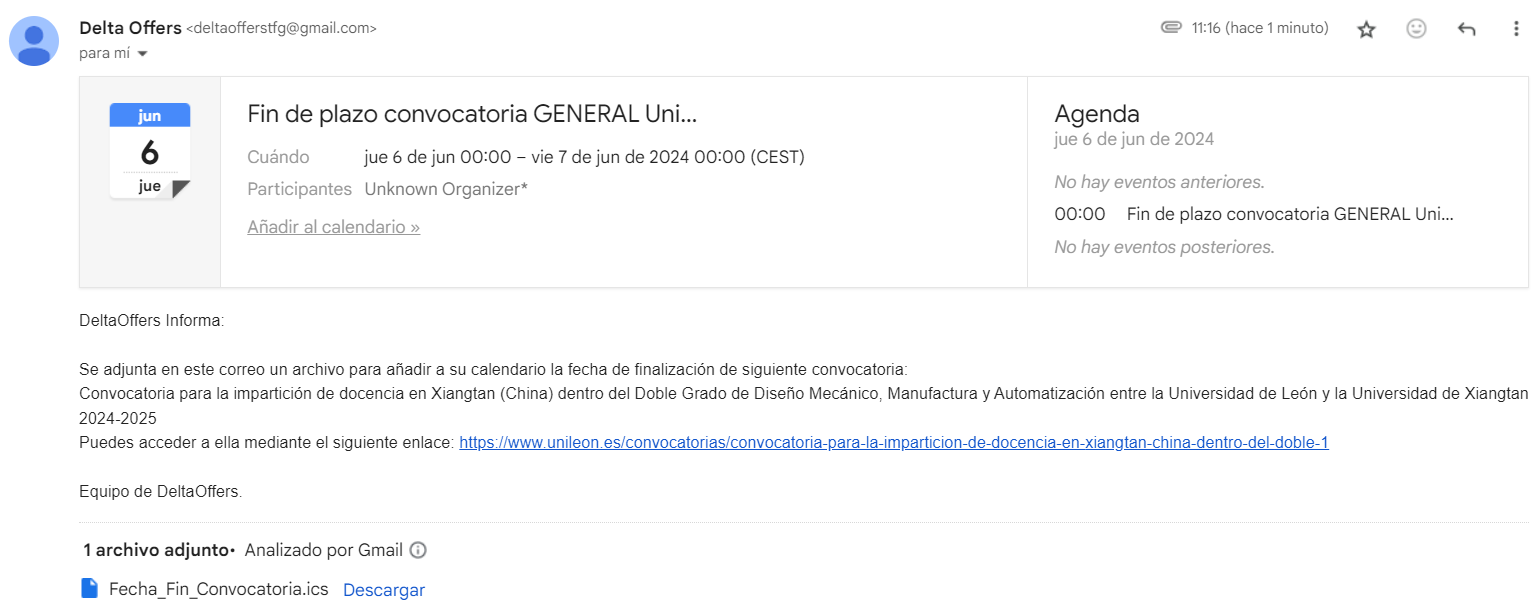
\includegraphics[width=1\linewidth]{DocumentacionTFG//img/AvisoCorreo.PNG}
    \caption{Correo enviado con archivo ICalendar adjunto}
    \label{fig:enter-label}
\end{figure}

Si el usuario finalmente desease añadir el fin de plazo de la convocatoria como evento en su calendario, deberá hacer \textit{click} en el apartado en el que pone 'Añadir al calendario'. Finalizado todo este proceso, el evento en el calendario aparecería de la siguiente manera:

\begin{figure}[H]
    \centering
    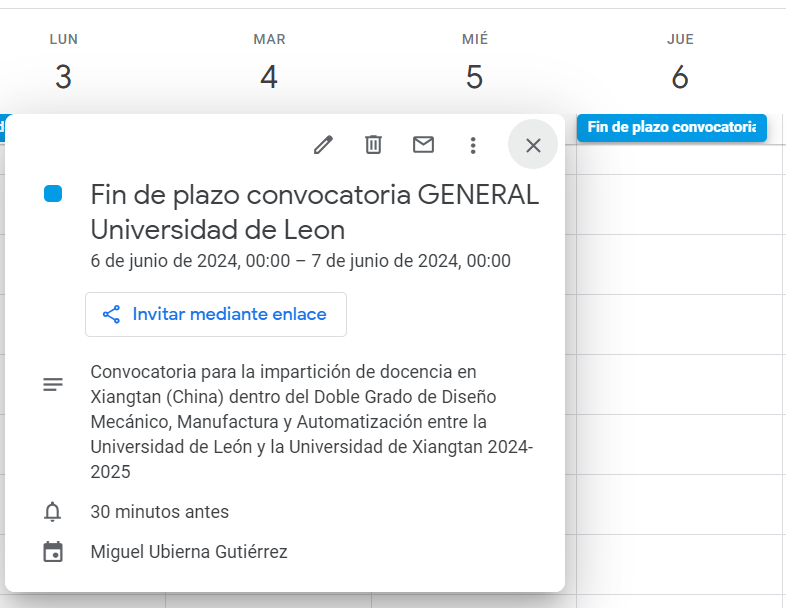
\includegraphics[width=0.6\linewidth]{DocumentacionTFG//img/EventoCalendario.PNG}
    \caption{Evento en calendario personal}
    \label{fig:evento-calendario}
\end{figure}

\subsection{Ver detalles}
Tal como se indicó en este apartado \ref{convocatoria-especifica}, para una convocatoria especifica, el usuario dispone de un botón 'Ver detalles' en la que se muestran detalles de la misma.

En este apartado de detalles, aparecerán otros datos e información de las convocatorias que no se mostraba en la ventana maestra en la que aparecía el listado. De esta manera, se proporcionará más información útil al usuario que esté interesado en una determinada convocatoria.

Los datos que podrás ver en esta ventana que anteriormente no se habían mostrado son:
\begin{itemize}
\item Descripción
\item Convocante
\item Fecha publicación
\item Destinatarios
\item Tipo
\item Clasificación
\item Nombre plaza
\item Convocatoria asociada
\end{itemize}

\textit{NOTA: Los campos mostrados en esta ventana, varían en función de la Universidad}

\begin{figure}[H]
    \centering
    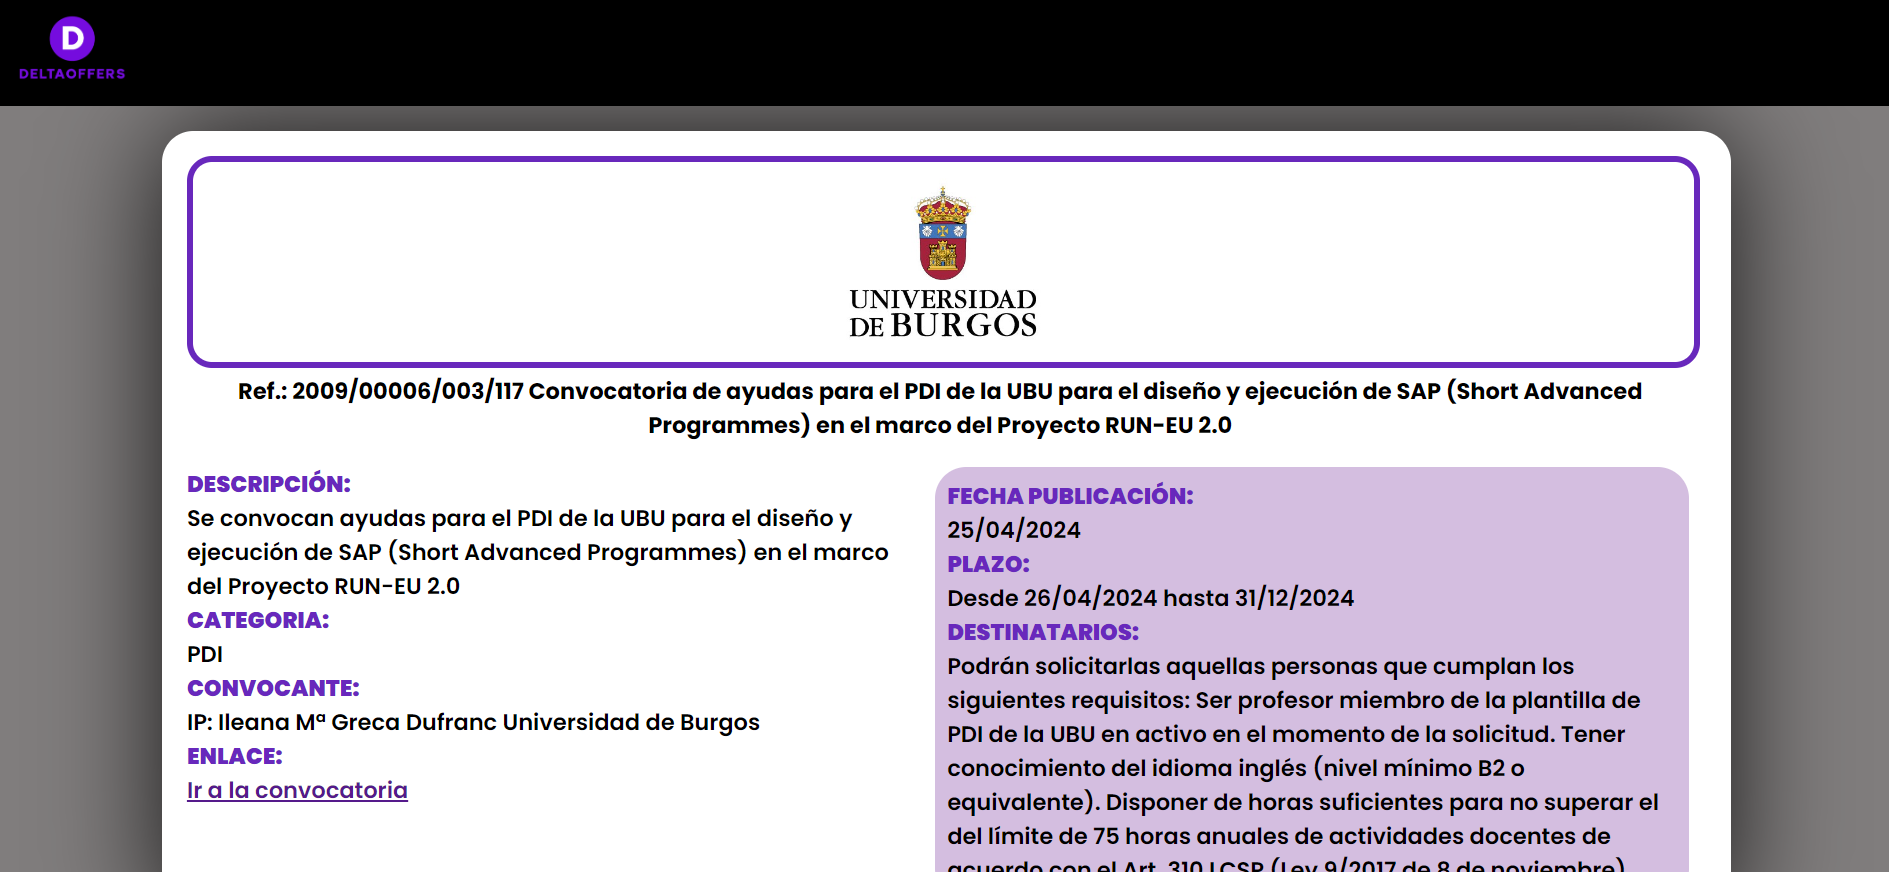
\includegraphics[width=1\linewidth]{DocumentacionTFG//img/Detalles.PNG}
    \caption{Ventana detalles}
    \label{fig:ventana-detalles}
\end{figure}

Además, desde la ventana de detalles, se dispone de un enlace a la convocatoria publicada en la web de la correspondiente universidad. De esta manera, los usuarios a los que les interese una convocatoria y quieran postularse como candidatos, podrán hacerlo mediante el enlace proporcionado.

\begin{figure}[H]
    \centering
    
\includegraphics[width=1\linewidth]{DocumentacionTFG//img/ConvocatoriaWebUniversidad.PNG}
    \caption{Convocatoria en la web de una universidad determinada}
    \label{fig:convocatoria-web-universidad}
\end{figure}